\documentclass[tikz, border=2pt]{standalone}
\usepackage{tikz}
\usetikzlibrary{arrows.meta,positioning,fit,backgrounds,calc,shapes.geometric}
% Shared TikZ style, color-matched to paper/figures/*.pdf (matplotlib):
% ink = near-black strokes/fill, accent = deep red for the one thing per
% diagram that should draw the eye, grid = light gray for structure that
% should recede.
\definecolor{ink}{HTML}{1A1A1A}
\definecolor{accent}{HTML}{A6192E}
\definecolor{gridgray}{HTML}{D9D9D9}
\definecolor{panelbg}{HTML}{F2F2F2}

\tikzset{
  every node/.style={font=\sffamily},
  box/.style={draw=ink, thick, rounded corners=1.5pt, minimum height=0.75cm,
              font=\sffamily\small, align=center, fill=white, text=ink},
  stubbox/.style={box, draw=ink, dashed, fill=panelbg},
  hibox/.style={box, fill=ink, text=white},
  panel/.style={draw=none, fill=panelbg, rounded corners=2pt},
  arr/.style={-{Latex[length=2.2mm, width=1.6mm]}, thick, draw=ink},
  darr/.style={arr, dashed},
  accarr/.style={-{Latex[length=2.2mm, width=1.6mm]}, thick, draw=accent},
  lbl/.style={font=\sffamily\scriptsize, text=ink},
  ital/.style={font=\sffamily\itshape\scriptsize, text=ink!70},
  note/.style={font=\sffamily\scriptsize, align=left, text=ink},
  state/.style={draw=ink, thick, rounded corners=3pt, minimum width=2.6cm,
                minimum height=0.9cm, font=\sffamily\small, align=center, fill=white},
  finalstate/.style={state, fill=ink, text=white},
  abortstate/.style={state, draw=accent, thick, text=accent},
}

\tikzset{
  dec/.style={draw=ink, thick, diamond, aspect=2.6, align=center, font=\sffamily\scriptsize,
              fill=white, inner sep=2pt, text width=2.5cm},
  term/.style={box, fill=ink!6},
}
\begin{document}
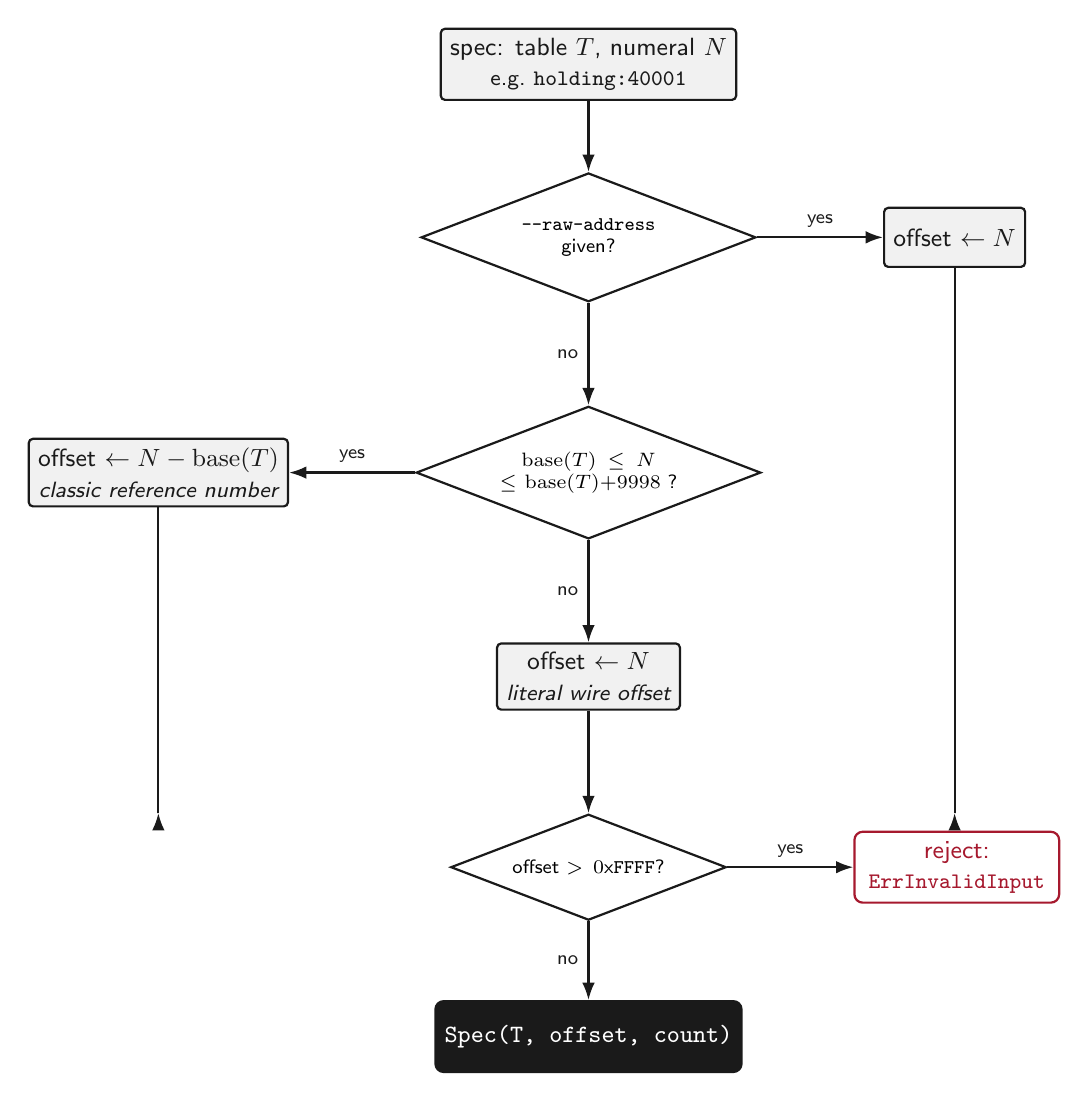
\begin{tikzpicture}[node distance=9mm and 9mm]

\node[term] (start) {spec: table \(T\), numeral \(N\) \\ \footnotesize e.g.\ \texttt{holding:40001}};
\node[dec, below=of start] (rawflag) {\texttt{-{}-raw-address} \\ given?};
\node[term, right=16mm of rawflag] (israw) {offset \(\leftarrow N\)};

\node[dec, below=13mm of rawflag] (inband) {\(\mathrm{base}(T) \le N \)\\ \(\le \mathrm{base}(T){+}9998\) ?};
\node[term, left=16mm of inband] (classic) {offset \(\leftarrow N - \mathrm{base}(T)\) \\ \footnotesize\itshape classic reference number};
\node[term, below=13mm of inband] (literal) {offset \(\leftarrow N\) \\ \footnotesize\itshape literal wire offset};

\node[dec, below=13mm of literal] (range) {offset \(> 0\)x\texttt{FFFF}?};
\node[abortstate, right=16mm of range] (err) {reject: \\ \footnotesize \texttt{ErrInvalidInput}};
\node[finalstate, below=10mm of range] (ok) {\texttt{Spec(T, offset, count)}};

\draw[arr] (start) -- (rawflag);
\draw[arr] (rawflag) -- node[lbl, above]{yes} (israw);
\draw[arr] (israw) |- (range.north -| israw);
\draw[arr] (rawflag) -- node[lbl, left]{no} (inband);
\draw[arr] (inband) -- node[lbl, above]{yes} (classic);
\draw[arr] (classic) |- (range.north -| classic);
\draw[arr] (inband) -- node[lbl, left]{no} (literal);
\draw[arr] (literal) -- (range);
\draw[arr] (range) -- node[lbl, above]{yes} (err);
\draw[arr] (range) -- node[lbl, left]{no} (ok);

\end{tikzpicture}
\end{document}
